\section{Matlab程序设计和GUI设计\scite{2}}
Matlab是一个功能极其强大的数据处理软件,传统的数据分析和处理都是人工计算,在面对一些复杂的计算时,会耗费大量的时间和精力,这就使效率低下。利用计算机进行数据处理,可以将一些重复的、复杂的计算快速准确地进行。利用计算机处理数据,除了可以省时省力外,可以将做过一次数据处理的源码保存下来,下一次进行同类型数据处理的时候可以重复利用。Matlab不仅仅可以进行数据处理,它还支持人机交互界面的设计,也就是Matlab的图形用户界面GUI(Graphical User Interface)。这就使得数据处理变的直观,非专业人士也可以轻松地使用别人开发好的GUI数据处理程序来完成一些数据的分析与处理。
\subsection{Matlab基本操作}
\subsubsection{Matlab的数据基础}
在Matlab软件中,用数组和cell数组的形式来存储任何数据,所有的数据处理是基于变量的操作。
\begin{enumerate}
	\item \textbf{数组}
	\begin{enumerate}
		\item 一维数组
		
		\qquad 数组就是数据的有序集合,一维数组可以看成向量,在处理的时候可以对一组有联系的数据以数组的形式赋值给变量。常用创建数组和获取数组数据的形式如下:
		\begin{lstlisting}
 >> a = [1 2 3 4 5];			% 直接输入创建一维数组,元素可以用空格或逗号隔开
    a = 
		1	2	3	4	5
 >> b = 1:2:9;					% 利用start:step:end 形式创建一维数组
	b =
		1	3	5	7	9
 >> a(3)						% 用变量名加下标的形式获取数组元素
 	ans = 
 		3\end{lstlisting}
		\item 二维数组
		
		\qquad 二维数组可以作为矩阵,在一维数组上增加一具维度,常用的创建和获取数组数据方法如下:
		\begin{lstlisting}
 >> a = [1 2 3;4 5 6;7 8 9]		% 直接输入创建二维数组,用“ ; ”换行
    a = 
    	1	2	3
    	4	5	6
    	7	8	9
 >> b = [1 2 3					% 直接输入创建二维数组,手动换行
 		 4 5 6
 		 7 8 9]
	b = 
	 	1	2	3
	 	4	5	6
	 	7	8	9
 >> a(2,2)						% 用变量名加下标来获取元素,二维数组用行数和列数来确定元素
 	ans = 
 		5\end{lstlisting}
	\end{enumerate}
	\item \textbf{cell数组}
	
	\qquad cell数组也是数组,它也可以是一维和二维,它的特殊之处就是它可以存放任何数据,也就是说它的元素可以是字符串,单个数据,甚至是数组。cell数组的使用方法如下:
	\begin{lstlisting}
 >> a = [1 2 3 4 5];				% 创建一维数组
 >> b = [1 2 3;4 5 6;7 8 9];		% 创建二维数组
 >> c = 'hello';					% 创建字符串
 >> d = {a,b,c}						% 赋值给 cell 数组
 	d = 
 		[1x5 double]	[3x3 double]	'Hello'
 >> d(1)							% 获取元素用“ ( ) ”,不能获取内容
 	ans =
 		[1x5 double]
 >> d{1}							% 获取元素内容用“ { } ”
 	ans =
 		1	2	3	4	5\end{lstlisting}
\end{enumerate}
\subsubsection{Matlab常用函数}
Matlab计算功能之所以强大,是因为它拥有很多的工具箱,里面封装了许多用于处理数据的函数,掌握如何使用这些函数,就掌握了Matlab的使用。在误差理论与数据处理中,常用的Matlab函数如下表:
\begin{figure}[H]
	\centering
	\begin{tabular}{p{3cm}<{\centering}p{8cm}}
		\toprule
		\textbf{函数}&\multicolumn{1}{c}{\textbf{作用}}	\\
		\midrule
		length(a)	&获取一维数组的长度\\
		size(A)	&获取二维数组的行与列\\
		max(A)	&获取数组A的最大值\\
		min(A)	&获取数组A的最小值\\
		mean(A)	&获取数组A的平均值\\
		sqrt(n)	&获取数值n的算术平方根\\
		std(X)	&获取数据X的标准差\\
		inv(A)	&获取矩阵的逆矩阵\\
		floor(x)	&获取小于x的最大整数\\
		ceil(x)	&获取大于x的最小整数\\
		roundn(x,n)	&对x进行四舍五入,数据精度为$ 10^n $\\
		\bottomrule
	\end{tabular}
	\captionsetup{type=table}
	\caption{Matlab常用误差处理函数}
\end{figure}
\subsubsection{Matlab绘制图像}
无论是处理数据和误差分析,还是进行别的数学计算处理的时候,绘制函数图形能更直接地了解数据的特性,也可以更直接地描述出计算的结果。在Matlab中,绘制函数图形的功能也是很强大的。在Matlab中常用绘图方法:
\begin{lstlisting}
 >> x = 0:0.01:2*pi;					% 产生一组数据 x
 >> y = sin(x);							% 用 sin 函数产生 y
 >> plot(x,y,'-b')						% 绘制函数图像,‘ - ’设置线条类型,‘ b ’设置颜色
 >> grid on								% 设置显示网格
 >> title('the function of sin')		% 设置图像标题
 >> xlabel('x')							% 设置 x 坐标名称
 >> ylabel('y')							% 设置 y 坐标名称\end{lstlisting}
 绘制的结果如下图:
\begin{figure}[H]
	\centering
	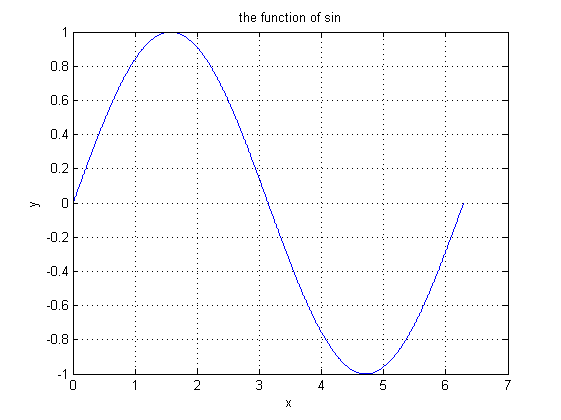
\includegraphics[scale=0.6]{sin_x}
	\caption{$ sin(x) $的函数图像}
\end{figure}
\subsubsection{Matlab的m文件}
Matlab编写的代码是以.m结尾的文件格式,m文件分为两种,m脚本文件和m函数文件。将执行的命令集写在m脚本文件中,直接在命令窗口输入文件名即可运行脚本文件,为了使文件不与Matlab自带的命令冲突,不要把文件命名与Matlab自带命令名称一致。编写脚本如下:
\begin{lstlisting}
   x = 0:0.01:2*pi;
   y = sin(x);
   plot(x,y,'-b')
   grid on
   title('the function of sin')
   xlabel('x')
   ylabel('y')\end{lstlisting}
将上面代码保存为plotsin.m文件,在命令窗口输入plotsin也可以绘制出图7函数图像。

还有一种是m函数文件,它在文件内部定义一个函数,由外界调取该函数进行计算,不可以单独运行,定义的函数名称要与文件名称一致,且不能与Matlab自带函数名称冲突。编写代码如下:
\begin{lstlisting}
 function sum = adds(x, y)
 sum = x + y;\end{lstlisting}
将上面代码保存为adds.m文件,在命令窗口输入adds(3,4),执行结果如下:
\begin{lstlisting}
 >> adds(3,4)
 	ans =
		 7\end{lstlisting}
\subsection{Matlab GUI设计}
在Matlab中,GUI设计有两种方法,一种是用代码实现界面的编程,还有一种是使用GUIDE图形界面设计,前者虽然编写代码量较大,界面的绘制都用代码实现,但在重复设计上有优势,比如大部分控件拥有相同的属性,在这里可以用循环来设置。后者虽然操作简单,界面绘制布局可视化,但在控件多的情况下,重复设置属性就比较麻烦了。在本毕业设计中,采用的前种设计方法。在Matlab中图形界面的层次结构\footnote{引用参考文献[2]第9章Matlab GUI的组成与结构第183页}如下图:
\begin{figure}[H]
	\centering
	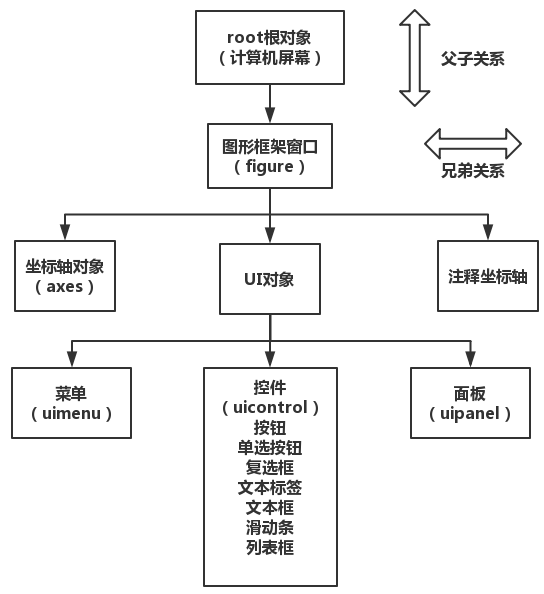
\includegraphics[scale=0.5]{MatlabGUI}
	\caption{GUI对象层次结构图}
\end{figure}
\subsubsection{Matlab中设计GUI的函数}
\begin{enumerate}
	\item \textbf{figure函数}

	\qquad 根据图8的结构图,设计图形界面首先要设计一个图形框架窗口,设计的方法如下:
	\begin{lstlisting}
 hf = figure('PropertyName',propertyvalue,...);\end{lstlisting}
 	其中:hf为对象名,函数的参数是成对存在的属性PropertyName和属性值propertyvalue,用来设置图形框架窗口的一些属性。比如执行如下代码:
	\begin{lstlisting}
 hf = figure('Name','MyFigure',...					% 设置窗口名称
    'NumberTitle','off',...							% 设置是否显示窗口编号
    'Position',[200,200,600,450],...				% 设置窗口的位置和大小
    'MenuBar','none',...							% 设置是否显示自带菜单
    'Color','White',...								% 设置界面颜色
    'Resize','off');								% 设置界面大小是否可变\end{lstlisting}
	上面代码可以在命令窗口和m文件内执行,执行结果如下图:
	\begin{figure}[H]
		\centering
		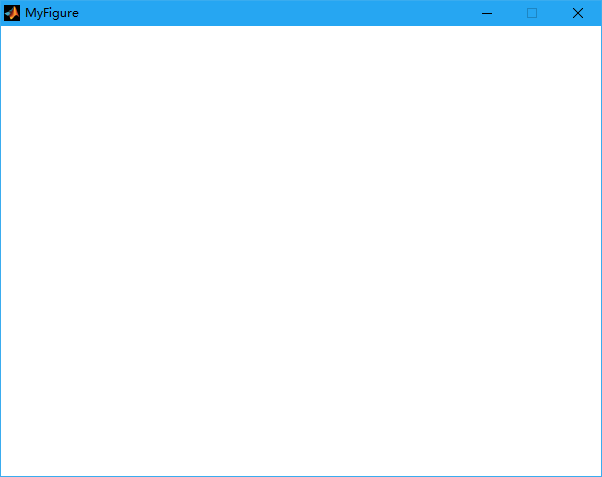
\includegraphics[scale=0.4]{MyFigure}
		\caption{MyFigure窗口}
	\end{figure}
	根据图9的结果,窗口的位置和大小都是固定的,而且窗口是不可变的,不能拖拽放大,也不能最大化,因为在属性中设置的结果。
	\item \textbf{uimenu函数}

	\qquad 在设计菜单的时候,必须要先有一个图形框架窗口,在前面用figure函数\footnote{参考文献[2]第9章Matlab GUI的组成与结构第183页}创建好的界面基础上设计菜单栏。设计的方法如下:
	\begin{lstlisting}
 hm = uimenu(parent,'PropertyName',propertyvalue,...);\end{lstlisting}
	其中:hm为对象名,参数parent为父对象名,后面的参数同样是成对存在的属性PropertyName和属性值propertyvalue,用来设置菜单的一些属性。执行如下代码:
	\begin{lstlisting}
 hm1 = uimenu(hf,'label','菜单1');
 hm2 = uimenu(hf,'label','菜单2');
 hm3 = uimenu(hf,'label','菜单3');
 subhm1 = uimenu(hm2,'label','子菜单1');
 subhm2 = uimenu(hm2,'label','子菜单2');
 subhm3 = uimenu(hm2,'label','子菜单3');\end{lstlisting}
 	参数parent是父对象,当父对象为菜单时,创建下拉子菜单。运行结果如图10。
	\item \textbf{uicontrol函数}
	
	\qquad 创建常用的控件使用uicontrol函数,常用的控件有按钮、静态文本、文本框、单选框、多选框等等。uicontrol函数\footnote{参考文献[2]第9章Matlab GUI的组成与结构第199页}如下:
	\begin{lstlisting}
 ui = uicontrol(parent,'PropertyName',propertyvalue,...);\end{lstlisting}
 	其中的参数属性设置与前面的一样。
	\begin{figure}[H]
		\centering
		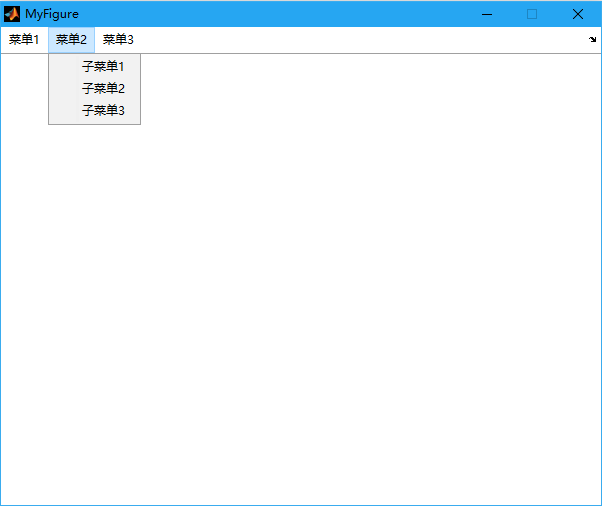
\includegraphics[scale=0.35]{MyFigure_uimenu}
		\caption{带菜单的MyFigure窗口}
	\end{figure}
	继续添加如下代码运行测试,运行结果为图11。
	\begin{lstlisting}
 ui = 1:4;												% 创建控件数组
 string = {'text','edit','pushbutton','popup'};			% 创建控件名称字符串数组
 position = [100,380,240,25								% 创建位置和大小的二级数组
             100,350,240,25
 			 100,320,240,25
             100,290,240,25];
 for i = 1:length(ui)									% 利用 for 循环创建控件和设置属性参数
     ui(i) = uicontrol(hf,...							% 设置父对象
         'Style',string{i},...							% 设置控件类型,调用 string 数组
         'FontSize',10,...								% 设置字体大小
		 'Tag',string{i},...							% 设置 Tag 标签
         'Units','pixels',...							% 设置位置大小设置类型为像素
         'String',string{i},...							% 设置显示的字符串
         'Position',position(i,:));						% 设置位置和大小,调用二维数组
 end\end{lstlisting}
 	\begin{figure}[H]
		\centering
		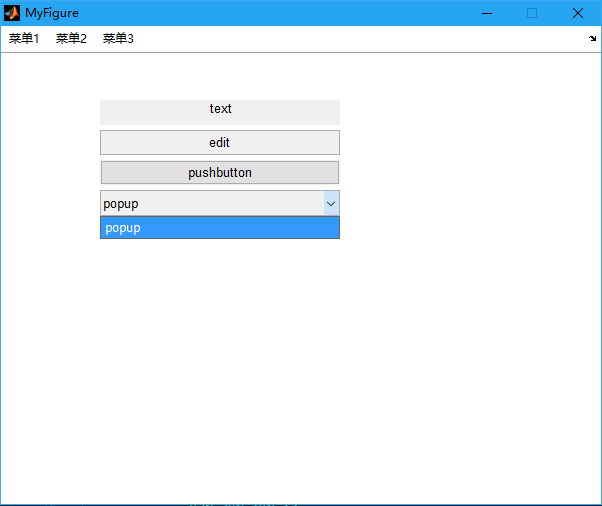
\includegraphics[scale=0.35]{MyFigure_uicontrol}
		\caption{带控件的MyFigure窗口}
	\end{figure}
	以后界面中的控件设计就用此函数实现,利用for循环和定义属性值数组可以更灵活的创建控件和设置控件的属性。该毕业设计的界面控件设计就是利用此方法来实现控件的布局和大小设置。
	\item \textbf{uipanel函数}

	\qquad uipanel函数\footnote{参考文献[2]第9章Matlab GUI的组成与结构第203页}可以创建一个面板来使控件归类,使界面的控件设计更直观,实现的函数如下:
	\begin{lstlisting}
 ui = uipanel(parent,'PropertyName',propertyvalue,...);\end{lstlisting}
 	其中的参数属性设置和前面的函数一样。继续向前面的m文件中追加如下代码,运行结果如图12。
	\begin{lstlisting}
 up = uipanel(hf,...									% 设置父对象
 	'Title','uipanel',...								% 设置名称
 	'FontSize',10,...									% 设置字体大小
 	'Units','pixels',...								% 设置位置大小设置类型为像素
 	'Position',[100,100,350,160]);						% 设置位置和大小\end{lstlisting}
	\begin{figure}[H]
		\centering
		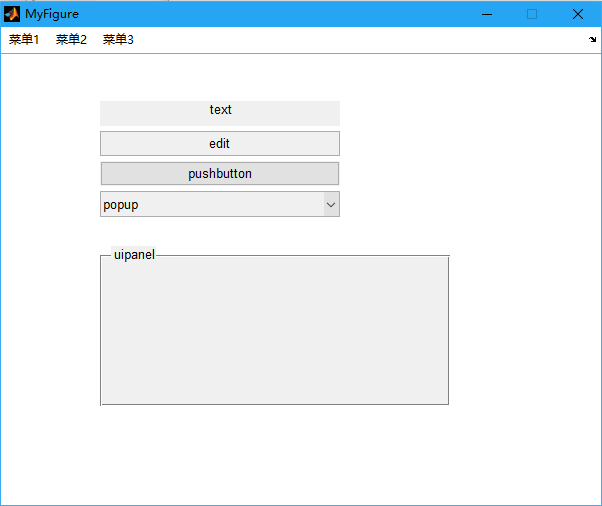
\includegraphics[scale=0.35]{MyFigure_uipanel}
		\caption{带面板的MyFigure窗口}
	\end{figure}
	\item \textbf{axes函数}

	\qquad 在界面设计的过程中,要想在界面上绘制函数图像,则必须创建axes坐标轴\footnote{参考文献[2]第9章Matlab GUI的组成与结构第218页},创建方法如下:
	\begin{lstlisting}
 ua = axes('PropertyName',propertyvalue,...);\end{lstlisting}
 	其中的参数属性设置和前面的函数一样。继续向前面的m文件中追加如下代码,运行结果如图13。
	 \begin{lstlisting}
 ua = axes(...											% 定义坐标轴对象名为 ua
	'Units','pixels',...								% 设置位置大小设置类型为像素
	'Position',[100,100,350,160]);						% 设置位置和大小
	x = 0:0.01:2*pi;
	y = sin(x);
	axes(ua);											% 设置绘图的坐标轴为 ua
	plot(x,y);\end{lstlisting}
	\begin{figure}[H]
		\centering
		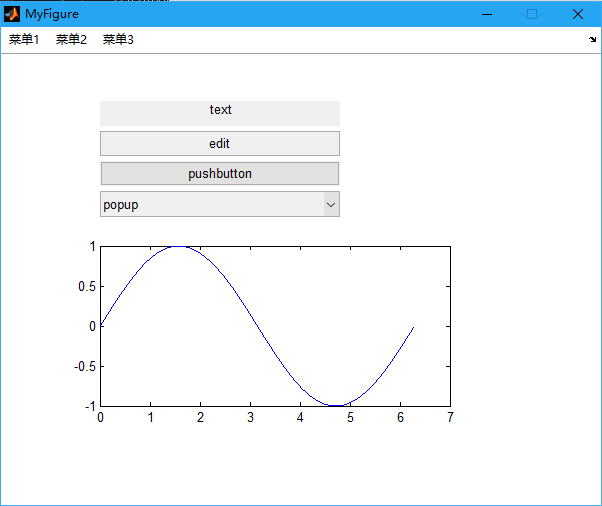
\includegraphics[scale=0.35]{MyFigure_axes}
		\caption{带坐标轴的MyFigure窗口}
	\end{figure}
\end{enumerate}

利用前面的5个GUI设计函数,可以设计出任何图形交互界面,只需要在函数参数中根据需求设置属性即可,控件中常用的属性设置见附录B,但上面的仅仅是设计好界面,还不能够处理数据,要想使用控件触发事件,则需要使用回调函数。
\subsubsection{Matlab中回调函数的编写}
GUI界面中,要想实现数据的交互和计算处理,要用到下面三个函数来获取界面控件属性的值和设置界面控件的属性。
\begin{enumerate}
	\item \textbf{get函数}

	\qquad 使用get函数可以获取对象的属性值,get函数的形式如下:
	\begin{lstlisting}
 get(h,'PropertyName');\end{lstlisting}
 	其中:h为要获取的对象,可以是控件、菜单、窗口等,PropertyName为要获取属性值的属性名称。在前面的代码中添加下面代码:
	 \begin{lstlisting}
 get(ui(3),'String')									% 获取 ui(3) 控件的 String 属性\end{lstlisting}
 	因为上面代码没有写分号,运行结果会在命令窗口输出pushbutton,因为ui(3)是之前创建的按钮控件。
	\item \textbf{set函数}

	\qquad 使用set函数可以设置对象的属性值,set函数的形式如下:
	\begin{lstlisting}
 set(h,'PropertyName',propertyvalue,...);\end{lstlisting}
 	其中:h为要设置的对象,可以是控件、菜单、窗口等,PropertyName为要设置属性的名称,propertyvalue为要设置的属性值。在前面的代码中添加下面代码:
	 \begin{lstlisting}
 set(ui(1),'String',1);									% 设置 ui(1) 控件的 String 属性为1\end{lstlisting}
 	运行结果可以发现界面中text已经变成1了,因为创建的ui(1)为静态文本控件。
	\item \textbf{guidata函数}

	\qquad 这个函数可以用来存储和获取GUI界面的控件数据,每个控件在Matlab中都有一个ID,主界面的所有控件ID都存放在一个数组里,guidata函数可以将ID以结构体的形式保存起来,结构体中有控件的Tag属性和ID,然后可以在回调函数中利用guidata函数来获取需要设置的控件。将前面的代码改成m函数文件,再添加如下代码:
	\begin{lstlisting}
 function MyFrame										% 创建 m 函数文件,名称与文件名称一致
 hf = figure('Name','MyFigure',...						% 省略前面写好的代码
 ......
 set(ui(3),'Callback',@fun_plot);						% 设置按钮的回调函数为fun_plot
 guidata(hf,guihandles);								% 将控件 guihandles 保存在窗口对象变量 hf 中

 function fun_plot(cbo,handles)							% 创建回调函数
 handles = guidata(cbo)									% 根据按钮来获取前面保存的数据
 set(handles.text,'String',2);							% 设置 text 的 String 属性为2\end{lstlisting}
 	运行上面的函数文件,然后单击按钮,就会在命令窗口打印下面的信息,它是所有带Tag属性控件的结构体,信息包含控件Tag和ID,单击按钮后还会使text的String属性变成2。设置和获取属性时用handles.Tag来获取控件。
	\begin{lstlisting}
 handles = 
         popup: 9.0455
    pushbutton: 8.0455
          edit: 7.0455
          text: 6.0455\end{lstlisting}
\end{enumerate}

通过设置回调函数,设置界面控件数据的保存和读取,可以完成界面处理数据的功能。在基于GUI的误差理论与数据处理设计中,先设计好界面,然后再设计数据处理的m文件,然后可以通过回调函数来调用它们。界面设计的部分代码见附录C,数据处理的部分代码见附录D,项目源代码:\url{https://github.com/AiJiangnan/ErrorTheoryDataProcessing}